\documentclass[a4paper,9pt]{article}
\usepackage{fontspec}
\setmainfont{Helvetica Neue}[
  BoldFont=Helvetica Neue Bold,
  ItalicFont=Helvetica Neue Italic
]
\usepackage[top=18mm, bottom=15mm, left=18mm, right=18mm]{geometry}
\usepackage{parskip}
\setlength{\parskip}{3pt}
\setlength{\parindent}{0pt}
\usepackage{xcolor}
\definecolor{primary}{HTML}{2563EB}
\definecolor{darkbg}{HTML}{0A0F1E}
\definecolor{bodytext}{HTML}{374151}
\definecolor{heading}{HTML}{0A0F1E}
\definecolor{subtitle}{HTML}{64748B}
\definecolor{lightgray}{HTML}{F8F9FA}
\definecolor{gold}{HTML}{C8AA50}
\definecolor{lightblue}{HTML}{EFF6FF}
\usepackage{titlesec}
\titleformat{\section}{\fontsize{11}{13}\selectfont\bfseries\color{heading}}{}{0em}{}[\vspace{-4pt}]
\titlespacing*{\section}{0pt}{6pt}{2pt}
\usepackage{tabularx}
\usepackage{booktabs}
\usepackage{colortbl}
\usepackage{enumitem}
\setlist[itemize]{leftmargin=1em, itemsep=0pt, parsep=0pt, topsep=1pt, label={\color{primary}\textbullet}}
\usepackage{hyperref}
\hypersetup{colorlinks=true, linkcolor=primary, urlcolor=primary}
\usepackage{tikz}
\usetikzlibrary{calc}
\usepackage{multicol}
\usepackage{microtype}
\pagestyle{empty}
\color{bodytext}

\begin{document}

% HEADER BAR
\begin{tikzpicture}[remember picture, overlay]
  \fill[darkbg] ($(current page.north west)$) rectangle ($(current page.north east)+(0,-2.2cm)$);
  \node[anchor=west, text width=12cm] at ($(current page.north west)+(1.8cm,-1.1cm)$) {
    {\fontsize{16}{18}\selectfont\bfseries\color{white}48 Hours with an AI Co-Pilot}
    \hfill
    {\fontsize{8}{10}\selectfont\color{gold}Florian Ziesche · Ainary Ventures · Feb 6--7, 2026}
  };
\end{tikzpicture}

\vspace{14mm}

{\fontsize{8.5}{11}\selectfont\color{subtitle}One person. One AI agent. 48 hours. No team. No contractors. No templates. The AI runs continuously while the human directs strategy and reviews output.}

\vspace{2pt}

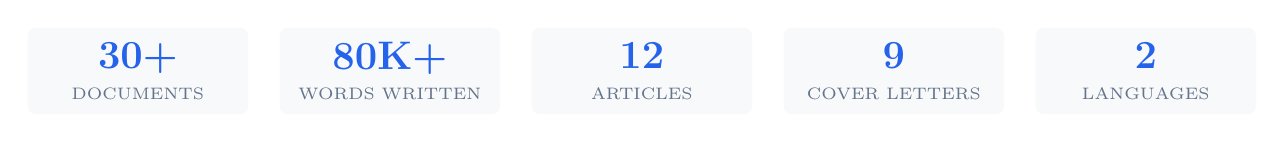
\begin{tikzpicture}
  \foreach \val/\lab/\xpos in {30+/Documents/0, 80K+/Words Written/3.2, 12/Articles/6.4, 9/Cover Letters/9.6, 2/Languages/12.8} {
    \node[fill=lightgray, rounded corners=3pt, minimum width=2.8cm, minimum height=1.1cm, inner sep=3pt, align=center] at (\xpos,0) {
      {\fontsize{14}{16}\selectfont\bfseries\color{primary}\val}\\[-1pt]
      {\fontsize{6}{8}\selectfont\color{subtitle}\MakeUppercase{\lab}}
    };
  }
\end{tikzpicture}

\vspace{4pt}
{\color{lightgray!70!white}\rule{\linewidth}{0.3pt}}
\vspace{2pt}

\begin{multicols}{2}
\fontsize{8}{10.5}\selectfont

\section{Professional Documents}
\begin{itemize}
  \item \textbf{Redesigned CV} — LaTeX PDF, brand-consistent, VC-optimized
  \item \textbf{9 personalized cover letters} — tailored to each firm's thesis and portfolio
  \item \textbf{2 application portals} researched with step-by-step submission guides
\end{itemize}

\section{Full Website (from scratch)}
\begin{itemize}
  \item \textbf{Bilingual} (EN + DE) — dark/gold design, 7 sections
  \item \textbf{6 service categories}: Manufacturing, Media, Legal, Operations, Workshops, Advisory
  \item \textbf{Full SEO}: Open Graph, Twitter Cards, JSON-LD, 20+ hyperlinks
  \item \textbf{Interactive journal} with 5 embedded articles
  \item \textbf{AI lead-gen CTA}: ``Ask my AI if we can build your use case''
  \item Mobile-responsive, works offline
\end{itemize}

\section{12 Articles Written}
\begin{itemize}
  \item \textbf{5 original articles} (EN) — AI architecture, human-AI collaboration, applied research
  \item \textbf{5 German translations} — natural rewrites, not machine translation
  \item \textbf{1 newspaper demo} — regional daily voice, local stats, balanced reporting
  \item \textbf{1 opinion piece on Sequoia's AGI thesis} (2,200 words) — 3-agent process: Research + Writer + Red Team → synthesized final
\end{itemize}

\section{Strategic \& Research Output}
\begin{itemize}
  \item \textbf{Blog content strategy} (v2) — multi-agent research + adversarial review
  \item \textbf{Business pitch} — 3-stage AI pilot proposal for major media group
  \item \textbf{VC positioning analysis} (25K words) — content strategy for career transition
  \item \textbf{Red team analysis} — systematic self-critique, 3 vulnerabilities found, thesis reframed
  \item \textbf{9 personalized sales emails} — researched, written, ready to send
  \item \textbf{Deployment analysis} — 3 hosting options compared
\end{itemize}

\section{How It Works}

The human directs. The AI executes — in parallel:

\begin{itemize}
  \item \textbf{Researches}: web search, source synthesis, competitive analysis
  \item \textbf{Writes}: articles, emails, pitches in calibrated voice
  \item \textbf{Builds}: websites, PDFs, dashboards
  \item \textbf{Challenges itself}: adversarial agents find weaknesses
  \item \textbf{Organizes}: file sync, memory, briefings
\end{itemize}

\vspace{3pt}
{\color{lightgray!70!white}\rule{\linewidth}{0.3pt}}
\vspace{3pt}

\textbf{The validated process:}\\[2pt]
\textbf{1.} Fast first draft → \textbf{2.} 3 parallel research agents → \textbf{3.} Human synthesis → \textbf{4.} v1 vs v2 comparison

\vspace{4pt}

\colorbox{lightblue}{\parbox{\dimexpr\linewidth-8pt}{%
\fontsize{8}{10.5}\selectfont\color{darkbg}
\textbf{The key insight:} The AI doesn't replace judgment. It amplifies capacity. Strategy stays human. Execution scales through AI.
}}

\end{multicols}

\vspace{2pt}
{\color{lightgray!70!white}\rule{\linewidth}{0.3pt}}
\vspace{1pt}
\begin{center}
{\fontsize{7}{9}\selectfont\color{subtitle}Florian Ziesche — AI Consultant \& VC Lab Fellow · \href{https://ainaryventures.com}{ainaryventures.com} · \href{mailto:f.ziesche.us@gmail.com}{f.ziesche.us@gmail.com}}
\end{center}

\end{document}
